% Conditional IUI draft generated from pipeline/CONDITIONAL_PAPER.md.
% Regenerate with the command documented in pipeline/BUILD.md.
\documentclass[manuscript,review,anonymous]{acmart}

\AtBeginDocument{\providecommand\BibTeX{{Bib\TeX}}}
\setcopyright{none}
\settopmatter{printacmref=true, printccs=true, printfolios=true}
\renewcommand\footnotetextcopyrightpermission[1]{}

\usepackage{amsmath}
\usepackage{array}
\usepackage{booktabs}
\usepackage{graphicx}
\usepackage{xcolor}
\usepackage{tikz}
\usetikzlibrary{arrows.meta,positioning,shapes.geometric}

\providecommand{\tightlist}{%
  \setlength{\itemsep}{0pt}\setlength{\parskip}{0pt}}
\newcommand{\Gap}[1]{\textcolor{red}{[MISSING FACT: #1]}}
\newcommand{\TopRule}{\toprule}

\begin{document}

\title{When Does a Legible Latent Axis Earn a Control? A Comparator-Bound Evaluation Contract for Latent-Control Interfaces}
\renewcommand{\shorttitle}{When Does a Legible Latent Axis Earn a Control?}

\author{Anonymous Authors}
\affiliation{%
  \institution{Anonymous Institution}
  \city{}
  \country{}
}

\begin{abstract}
% Provisional model-evidence abstract; revise only after a gated pending-study decision.
Interfaces increasingly place controls beside named latent properties, implying that moving the control will reliably change the corresponding behavior. Readable directions and changed outputs do not establish that promise when prompting already provides a behavioral alternative. We contribute a comparator-bound evaluation contract: READ records local representational support; TRANSFER tests behavioral improvement over a declared prompt comparator; and the comparator, calibration warning, and evidence tier preserve what the interface can claim. We instantiate the contract with a DEV-selected prompt drawn from a preregistered bounded candidate set across Qwen and Llama, CAA and ITI, and three behavioral axes. None of the 12 model--method--axis tests qualified under the reported rule, but the contract separates three actionable profiles: skepticism requires greater resolution, deliberation is mixed, and uncertainty favors the comparator under the frozen scorer while its all-generation interpretation remains open. A post hoc, author-proposed mapping translates these profiles into \emph{Diagnostic-only}, \emph{Unresolved}, \emph{Unstable}, and \emph{Eligible} affordance states. The worked application shows how a latent-control interface can turn heterogeneous model evidence into a specific design decision rather than a generic slider.
\end{abstract}

\begin{CCSXML}
<ccs2012>
 <concept><concept_id>10003120.10003121.10011748</concept_id>
  <concept_desc>Human-centered computing~Empirical studies in HCI</concept_desc>
  <concept_significance>500</concept_significance></concept>
 <concept><concept_id>10003120.10003130.10011762</concept_id>
  <concept_desc>Human-centered computing~Collaborative and social computing theory, concepts and paradigms</concept_desc>
  <concept_significance>300</concept_significance></concept>
 <concept><concept_id>10010147.10010178.10010179</concept_id>
  <concept_desc>Computing methodologies~Natural language processing</concept_desc>
  <concept_significance>300</concept_significance></concept>
</ccs2012>
\end{CCSXML}
\ccsdesc[500]{Human-centered computing~Empirical studies in HCI}
\ccsdesc[300]{Human-centered computing~Collaborative and social computing theory, concepts and paradigms}
\ccsdesc[300]{Computing methodologies~Natural language processing}

\keywords{latent steering, mechanistic interpretability, intelligent user interfaces,
prompt comparator, evidence qualification, human--AI interaction}

\maketitle

% CONDITIONAL DRAFT — NOT FINAL NARRATIVE LOCK

% Human-study and prompt-plus-steer result slots remain empty and gated.

\section{Introduction}\label{introduction}

Alex is drafting a policy recommendation with an AI assistant and sees a slider labeled ``uncertainty awareness.'' Raising it appears to promise that the assistant will better distinguish what it knows from what it does not. The widget makes a behavioral claim. A readable direction or a changed completion does not show that the latent route improves the named outcome over instructions Alex could already give.

This is no longer a hypothetical interface pattern. Bo et al.~expose activation steering through SELECT, CALIBRATE, and LEARN controls, while Anthropic's Golden Gate Claude made interaction with an internally modified Claude 3 Sonnet publicly visible for 24 hours. \cite{bo2026steerable,anthropic2024goldengate} {}% SOURCE_CHECKED 2026-08-11
Karny et al.~further show that a neural-transparency interface can change reported trust and perceived helpfulness without changing several behavioral outcomes. \cite{karny2026neural} These precedents make the evidence behind an active latent control an interface question, not only a model-analysis question.

We ask: \textbf{what evidence should a latent-control interface require before a readable axis is presented as an actionable control?} We answer with a comparator-bound evaluation contract. READ records whether the label has local representational support. TRANSFER tests whether the intervention improves a declared behavioral outcome over a declared prompt comparator while satisfying an uncertainty rule, a 0.05 point-estimate floor, and coherence. The comparator, calibration warning, and evidence tier carry the result into the interface without transferring it across models, methods, axes, or tasks. {}% C-001
{}% C-002
{}% C-006

The worked application compares CAA and ITI on Qwen and Llama across deliberation, skepticism, and uncertainty awareness. The prompt comparator is selected on DEV from a preregistered bounded set of sixteen candidates; the latent coefficient is also selected on DEV, and the frozen settings enter paired TEST comparisons. {}% FL-002
{}% FL-008
{}% FL-031

None of the twelve model--method--axis tests qualifies under the reported rule. That common procedural result does not imply one common scientific state. Skepticism is underpowered near the point-estimate floor; deliberation is mixed; and uncertainty is negative relative to the comparator under the frozen scorer, with a targeted Qwen--CAA recheck whose complete-case estimate remains negative but whose all-generation missingness bounds cross zero. {}% FL-003
{}% FL-004
{}% FL-041
{}% FL-043
{}% FL-047
The contract preserves these differences instead of converting 0/12 into a universal null or a single interface verdict.

The reported rule determines pass or no-pass. Separately, an author-proposed post hoc mapping translates evidence profiles into four affordance states: \emph{Diagnostic-only}, \emph{Unresolved}, \emph{Unstable}, and \emph{Eligible}. {}% OI-014
In the worked uncertainty example, this mapping leads a design team to replace one active slider with a read-only diagnostic and comparator view.

% PENDING_HUMAN_STUDY_SLOT: Insert only a frozen preregistered result, including null/mixed/adverse/incomplete outcomes and caveat.

% PENDING_PROMPT_STEER_SLOT: Insert only frozen composition evidence; otherwise retain substitution-only scope.

This paper makes three contributions:

\begin{enumerate}
\def\labelenumi{\arabic{enumi}.}
\tightlist
\item
  \textbf{A comparator-bound qualification procedure for active latent controls.} It separates local READ evidence from behavioral TRANSFER evidence, reserves CONTROL for interface permission, and requires a declared alternative, outcome, uncertainty rule, point-estimate floor, coherence criterion, and evidence tier.
\item
  \textbf{A five-field interface record and state vocabulary.} The record preserves comparator, calibration, and scope through the proposed states \emph{Diagnostic-only}, \emph{Unresolved}, \emph{Unstable}, and \emph{Eligible}.
\item
  \textbf{A complete worked application.} The CAA/ITI by Qwen/Llama grid demonstrates how one procedural outcome separates into distinct interface decisions for limited resolution, mixed evidence, and comparator-relative calibration.
\end{enumerate}

Together, these contributions turn a familiar interface question into a versioned decision record: evidence first, affordance second.

\section{Related Work}\label{related-work}

\subsection{From Legible Representations to Behavioral Actionability}\label{from-legible-representations-to-behavioral-actionability}

Representation-engineering methods identify and intervene on directions inside language models. Representation Engineering centers population-level representations as objects for monitoring and manipulation; Activation Addition derives lightweight vectors from contrasting prompt pairs. \cite{zou2023repe,turner2023actadd} CAA estimates directions from paired positive and negative examples, while ITI derives probe directions and modifies activations during generation. \cite{rimsky2024caa,li2023iti} Instruction-specific vectors further show positive cases in which steering improves constraint following with and without explicit instructions. \cite{stolfo2025instr} {}% SOURCE_CHECKED 2026-08-11
Together, these methods establish that internal representations can be measured and manipulated under specified conventions. Our focus is the next interface decision: what behavioral evidence turns such a representation into a warranted control?

Recent benchmarks make this distinction empirically consequential. AxBench evaluates prompting, finetuning, and several representation-level methods on common concepts; its official Table 2 reports a mean overall steering score of 0.894 for Prompt and 0.239 for DiffMean after factor selection, distinct from the mutable repository leaderboard. \cite{wu2025axbench} {}% SRC-007
Basu et al.~examine the gap between internal representation and actionable output correction in 400 clinical vignettes, including a safety-focused prompt-engineering condition in Arm 1; for Qwen, sensitivity changes from 0.451 under the original parser to 0.729 under the refined parser, showing that the measured gap is parser-sensitive. \cite{basu2026actionability} {}% SRC-008
These studies establish the empirical premises for our contribution. We operate at the next unit of analysis: one proposed interface control, its declared comparator, and the evidence attached to its release decision.

Internal reach and behavioral advantage are distinct design quantities. Mishra et al.~show that steering can reach residual states outside a bounded prompt image. \cite{mishra2026nonsurj} Heyman and Vandeputte show that trained steering can mimic prompting, while Sprejer et al.~reveal capability--behavior trade-offs for feature steering relative to prompting. \cite{heyman2026steer,sprejer2026mindgap} Together, these results motivate a local behavioral qualification record rather than an inference from internal geometry alone.

Work on metacognitive demands and human-centered transparency frames exposed information relative to a task and decision. \cite{tankelevitch2024metacog,liao2024transparency} {}% SOURCE_CHECKED 2026-08-11
We operationalize that principle as READ, TRANSFER, and CONTROL: local representational evidence, comparator-bound behavioral evidence, and the resulting interface permission.

\subsection{Prompting as a Declared Behavioral Alternative}\label{prompting-as-a-declared-behavioral-alternative}

Prompting is both a practical interaction channel and a technical comparator. Prompt-derived AI instruments can reify intent as reusable direct-manipulation controls, while studies of non-expert prompt design show that constructing and evaluating prompts is itself difficult. \cite{riche2025aiinstr,zamfirescuPereira2023johnny} AxBench directly places prompting beside representation-level methods. {}% SRC-007
Bo et al.~compare steering interfaces with an unscaffolded prompt baseline and separately test prompting on top of steering before their user study. \cite{bo2026steerable} {}% SRC-009
Basu et al.~include prompt engineering within a set of mechanistic intervention arms. {}% SRC-008
These works make prompting an established comparison channel. Our contribution is to bind that channel to a per-affordance interface decision rather than rank steering methods globally.

Our comparator is deliberately described more narrowly than ``the prompt a user could already have typed.'' The procedure selects the prompt comparator on DEV from a preregistered bounded set of sixteen candidates. {}% FL-008
{}% FL-009

The current application uses substitution: the latent intervention replaces the selected prompt channel. {}% FL-015

\subsection{Mechanistic-Interpretability Interfaces and Human Evidence}\label{mechanistic-interpretability-interfaces-and-human-evidence}

HCI work has begun turning internal model representations into visible or manipulable interface elements. Bo et al.~instantiate three steering designs---SELECT, CALIBRATE, and LEARN---and report heterogeneous preferences in an exploratory within-subject study. \cite{bo2026steerable} {}% SRC-009
Other systems expose feature steering, attribution-guided intervention, or embedding manipulation to people. \cite{huang2025steering,labarta2026attribution,raval2026latman} {}% SOURCE_CHECKED 2026-08-11
This literature establishes latent representations as interaction objects. We contribute the qualification step that connects evidence about one such object to its control state.

Public demonstrations extend this trajectory beyond research prototypes. Anthropic altered the strength of an internal Golden Gate Bridge feature in Claude 3 Sonnet and made the modified model available through \texttt{claude.ai} for 24 hours. \cite{anthropic2024goldengate} {}% SOURCE_CHECKED 2026-08-11
Bo et al.~supply configurable steering interfaces; Golden Gate Claude supplies public exposure to an internally modified model. Our target is the evidence policy that follows these technical and interface precedents: what must one named control establish before it receives CONTROL permission?

Karny et al.~provide the closest verified interface and human-evidence neighbor. Their neural-transparency system projects a system prompt onto persona trait vectors and presents the predictions through an interactive sunburst before users chat with their configured model. In a controlled between-subjects study, the visualization increased endpoint trust and was rated helpful, but it did not produce significant differences in prompt iteration, resulting persona scores, message engagement, or confidence in predicting unintended behavior. \cite{karny2026neural} {}% SRC-010
They study passive prediction and explicitly leave active steering interfaces to future work. Their subjective/behavioral divergence also cautions against treating perceived usefulness as evidence that an interface improves actionability judgments.

Documentation frameworks such as model cards and datasheets demonstrate how structured records can bind claims to provenance, evaluation, and scope. \cite{mitchell2019modelcards,gebru2021datasheets} Internal algorithmic-audit frameworks add a process-oriented precedent: staged development decisions produce linked records across the system lifecycle. \cite{raji2020accountability} {}% SOURCE_CHECKED 2026-08-11
Our five-field record applies a related accountability move at the control-affordance level: it records READ, TRANSFER, comparator, calibration warning, and evidence tier for one proposed active latent control. These precedents motivate traceability at the level of one affordance; our contribution makes the record operational through a behavioral qualification rule and worked interface decision.

\begin{table*}[t]
\centering
\footnotesize
\setlength{\tabcolsep}{4pt}
\caption{Nearest neighbors and the interface decision each leaves open.}
\label{tab:novelty-neighbors}
\begin{tabular}{@{}p{0.22\textwidth}p{0.34\textwidth}p{0.36\textwidth}@{}}
\TopRule
Prior work & What it establishes & What remains for the present interface decision \\
\midrule
Huang and Lim \cite{huang2025steering} & A lay interface for SAE feature steering and persona construction. & Whether each visible feature carries comparative behavioral evidence sufficient for an active control. \\
Bo et al. \cite{bo2026steerable} & SELECT, CALIBRATE, and LEARN interfaces, an unscaffolded PROMPT baseline, and exploratory within-subject user evidence. & A per-affordance qualification against a declared selected comparator, with margin, coherence, warning, and evidence tier. \\
Karny et al. \cite{karny2026neural} & A passive neural-transparency interface with controlled human evidence and subjective/behavioral divergence. & When evidence licenses an active intervention rather than a prediction display. \\
Wu et al. (AxBench) \cite{wu2025axbench} & A method-level benchmark comparing prompting with multiple representation-level interventions. & A widget-level decision tied to matched items, a declared margin, coherence, and scope. \\
Basu et al. \cite{basu2026actionability} & A clinical representation-to-actionability study whose Arm 1 includes prompt engineering and whose gap is parser-sensitive. & A uniform per-affordance record that carries comparator and measurement limits into an interface state. \\
Riche et al.; Labarta et al.; Raval et al. \cite{riche2025aiinstr,labarta2026attribution,raval2026latman} & Prompt instruments, an expert activation-steering workflow, and concept-guided latent manipulation. & A prompt-versus-latent behavioral qualification procedure for one language-model control. \\
Mishra et al. \cite{mishra2026nonsurj} & Internal residual-state non-surjectivity under bounded prompts. & Whether internal reach yields superior behavior under the declared outcome and comparator. \\
Heyman and Vandeputte \cite{heyman2026steer} & Trained steering that mimics prompting. & New evidence for the trained method rather than transfer from the present naive additive setting. \\
Sprejer et al. \cite{sprejer2026mindgap} & Capability–behavior trade-offs for feature steering relative to prompting. & A preregistered CAA/ITI comparison on the present outcomes and an interface permission record. \\
Rimsky et al.; Li et al. \cite{rimsky2024caa,li2023iti} & The CAA and ITI intervention families. & Whether the tested implementations exceed the declared comparator while preserving coherence. \\
\bottomrule
\end{tabular}
\end{table*}

\subsection{Positioning Summary}\label{positioning-summary}

Prior work supplies manipulable representations, prompt-based control, and latent-facing interfaces. We connect these ingredients with a per-affordance qualification record that carries comparator, measurement warning, and evidence tier directly into the design decision. {}% OI-009

\section{Method}\label{method}

\subsection{Evidence Status and Study Overview}\label{evidence-status-and-study-overview}

Exact values trace to committed result artifacts, preregistrations, analysis code, and machine-readable paper manifests. Generated tables and figures rebuild from those artifacts without manual value edits. {}% OI-001

The method has two levels. First, a control-affordance qualification record specifies what evidence a proposed active latent control would need to claim actionability. Second, a computational application fills the record for CAA and ITI relative to a DEV-selected prompt comparator drawn from a preregistered bounded candidate set. The application crosses two model families, two steering methods, and three behavioral TRANSFER axes. {}% FL-002
READ is evaluated separately with exploratory CAA-style directions and includes a fourth, focus-related axis that is not part of the twelve-test TRANSFER denominator. {}% FL-036
{}% FL-042

\subsection{Five-Field Qualification Record}\label{five-field-qualification-record}

The record contains five fields.

\begin{enumerate}
\def\labelenumi{\arabic{enumi}.}
\tightlist
\item
  \textbf{READ} specifies the model, method, direction construction, layer, task, and measurement under which an internal axis is legible. READ is a diagnostic precondition, not behavioral evidence.
\item
  \textbf{TRANSFER} records the behavioral outcome, intervention, estimand, uncertainty, point-estimate floor, and coherence result.
\item
  \textbf{COMPARATOR} identifies the declared behavioral alternative, candidate set, and selection procedure. In this application it is a DEV-selected prompt drawn from a preregistered bounded set of sixteen candidates; the field preserves the provenance limits detailed below. {}% BD-009
\item
  \textbf{CALIBRATION WARNING} states which contrast is being interpreted---for example, steer versus prompt rather than steer versus an unsteered baseline---and records missingness or scoring threats that can reverse the reading.
\item
  \textbf{EVIDENCE TIER} binds the record to a model, method, axis, task, layer, protocol, and evidence status so that a result cannot silently transfer to another setting.
\end{enumerate}

The vocabulary maps each record to one of four affordance states. \emph{Diagnostic-only} retains READ evidence for inspection when TRANSFER is untested or clearly misses the behavioral criteria. \emph{Unresolved} marks inadequate resolution or incomplete identification. \emph{Unstable} marks a coherence failure. \emph{Eligible} requires every declared behavioral criterion to pass within the evidence tier. The status of this mapping is specified in Limitations. {}% FL-077
{}% OI-014

\begin{figure*}[t]
\centering
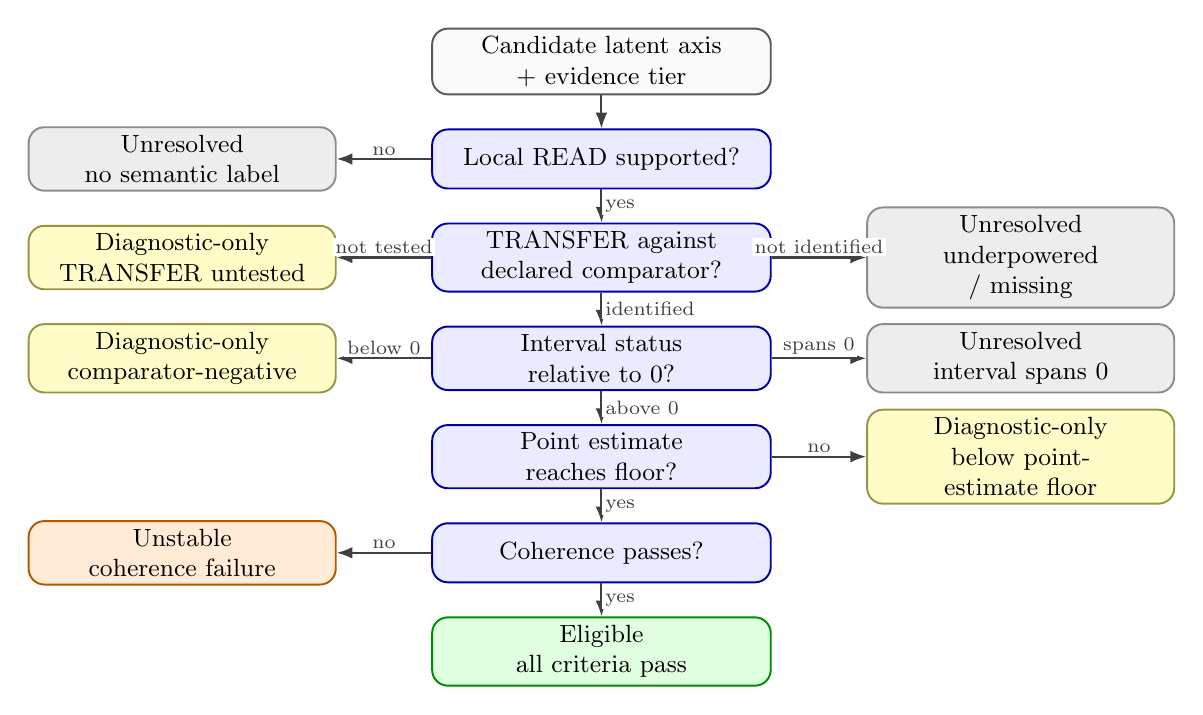
\begin{tikzpicture}[
    node distance=4.2mm and 12mm,
    base/.style={draw, rounded corners=2mm, align=center, minimum height=7.5mm,
        inner xsep=2.5mm, inner ysep=1mm, font=\small, line width=0.7pt},
    input/.style={base, text width=38mm, fill=black!2, draw=black!65},
    decision/.style={base, text width=38mm, fill=blue!8, draw=blue!65!black},
    unresolved/.style={base, text width=34mm, fill=black!7, draw=black!45},
    diagnostic/.style={base, text width=34mm, fill=yellow!22, draw=yellow!55!black},
    unstable/.style={base, text width=34mm, fill=orange!16, draw=orange!70!black},
    eligible/.style={base, text width=38mm, fill=green!12, draw=green!55!black},
    arrow/.style={-{Latex[length=2mm]}, line width=0.75pt, draw=black!75},
    flowlabel/.style={font=\scriptsize, fill=white, inner sep=1pt, text=black!75},
    branchlabel/.style={font=\scriptsize, fill=white, inner sep=1pt, text=black!75}
]
\node[input] (candidate) {Candidate latent axis\\+ evidence tier};
\node[decision, below=of candidate] (read) {Local READ supported?};
\node[unresolved, left=of read] (unresolvedread) {Unresolved\\no semantic label};
\node[decision, below=of read] (transfer) {TRANSFER against\\declared comparator?};
\node[diagnostic, left=of transfer] (diagnosticonly) {Diagnostic-only\\TRANSFER untested};
\node[unresolved, right=of transfer] (unresolvedtransfer) {Unresolved\\underpowered / missing};
\node[decision, below=of transfer] (interval) {Interval status relative to 0?};
\node[diagnostic, left=of interval] (comparatornegative) {Diagnostic-only\\comparator-negative};
\node[unresolved, right=of interval] (intervalopen) {Unresolved\\interval spans 0};
\node[decision, below=of interval] (floor) {Point estimate reaches floor?};
\node[diagnostic, right=of floor] (small) {Diagnostic-only\\below point-estimate floor};
\node[decision, below=of floor] (coherence) {Coherence passes?};
\node[unstable, left=of coherence] (coherencefailure) {Unstable\\coherence failure};
\node[eligible, below=of coherence] (eligiblecontrol) {Eligible\\all criteria pass};
\draw[arrow] (candidate) -- (read);
\draw[arrow] (read.west) -- node[branchlabel, above] {no} (unresolvedread.east);
\draw[arrow] (read) -- node[flowlabel, right] {yes} (transfer);
\draw[arrow] (transfer.west) -- node[branchlabel, above] {not tested} (diagnosticonly.east);
\draw[arrow] (transfer.east) -- node[branchlabel, above] {not identified} (unresolvedtransfer.west);
\draw[arrow] (transfer) -- node[flowlabel, right] {identified} (interval);
\draw[arrow] (interval.west) -- node[branchlabel, above] {below 0} (comparatornegative.east);
\draw[arrow] (interval.east) -- node[branchlabel, above] {spans 0} (intervalopen.west);
\draw[arrow] (interval) -- node[flowlabel, right] {above 0} (floor);
\draw[arrow] (floor.east) -- node[branchlabel, above] {no} (small.west);
\draw[arrow] (floor) -- node[flowlabel, right] {yes} (coherence);
\draw[arrow] (coherence.west) -- node[branchlabel, above] {no} (coherencefailure.east);
\draw[arrow] (coherence) -- node[flowlabel, right] {yes} (eligiblecontrol);
\end{tikzpicture}
\caption{Proposed evidence-to-affordance flow. Color distinguishes decisions (blue) from the four formal states: Diagnostic-only (yellow), Unresolved (gray), Unstable (orange), and Eligible (green). Text labels carry the same distinctions. Outputs retain comparator, warning, and evidence tier.}
\Description{A candidate axis first receives a local READ check. Unsupported READ routes to Unresolved. Supported READ proceeds to comparator-bound TRANSFER. Untested, comparator-negative, or below-floor evidence routes to Diagnostic-only; underpowered, missing, or zero-spanning evidence routes to Unresolved; coherence failure routes to Unstable; and a complete pass routes to Eligible within its evidence tier.}
\label{fig:evidence-flow}
\end{figure*}

\subsection{Models, Methods, and Behavioral Axes}\label{models-methods-and-behavioral-axes}

The worked application uses Qwen2.5-7B-Instruct and Meta-Llama-3-8B-Instruct, with the latter loaded from the NousResearch identical-weights mirror after gated access blocked the canonical repository. {}% FL-011
{}% MODEL_IDS: Qwen/Qwen2.5-7B-Instruct; NousResearch/Meta-Llama-3-8B-Instruct
Both run in CUDA float16. The committed artifacts record the selected hidden-state layers by deliberation/skepticism/uncertainty: Qwen--CAA uses 20/20/20, Qwen--ITI uses 20/19/17, Llama--CAA uses 12/14/10, and Llama--ITI uses 8/14/11. The intervention hooks the output of decoder block \(L-1\), which corresponds to Hugging Face hidden state \(L\), and adds the direction at every token position during prefill and generation. Activation extraction renders one user turn through the model chat template and pools the last non-padding token. Immutable upstream model revision hashes were not recorded.

CAA uses a positive-minus-negative mean-difference direction that is unit-normalized before injection. {}% FL-023
{}% FL-024
ITI fits a logistic probe to the same 28-pair extraction split, selects a nondegenerate layer no shallower than 20\% of model depth, unit-normalizes the probe direction, and multiplies it by the frozen projected-activation sample standard deviation. {}% FL-025
Both methods select a coefficient from \(\{2,4,6,8,12,16,24\}\) on DEV, but equal coefficients do not imply equal injected norms: ITI injects \(\alpha\sigma_L\), so no common norm bound of 24 applies. {}% FL-012
{}% FL-026

The reported CAA convention is

\begin{equation}
\begin{aligned}
v_a &= \mathbb{E}_{x\in A_a^+}[h_L(x)]-\mathbb{E}_{x\in A_a^-}[h_L(x)],\\
\hat v_a &= v_a/\lVert v_a\rVert, \qquad h'_L=h_L+\alpha\hat v_a.
\end{aligned}
\label{eq:caa-steering}
\end{equation}

The common additive notation preserves method-specific scale:

\begin{equation}
h'_L=h_L+\alpha s_{m,a,L}\hat u_{m,a,L},\qquad
s_{\mathrm{CAA},a,L}=1,\quad s_{\mathrm{ITI},a,L}=\sigma_{a,L}.
\label{eq:method-scaling}
\end{equation}

% FL-023–FL-026

Equations \ref{eq:caa-steering} and \ref{eq:method-scaling} make the method-specific scaling explicit.

The three TRANSFER axes use task accuracy for deliberation, false-premise rejection for skepticism, and \(1-\mathrm{Brier}\) for uncertainty awareness. {}% FL-018
These operational outcomes do not exhaust the psychological constructs named by the axes. For uncertainty, both conditions request an answer and confidence. The deterministic parser accepts \texttt{Confidence:}/\texttt{conf} forms, interprets values above one as percentages, clamps them to \([0,1]\), and imputes missing confidence as 0.5, which makes \(1-\mathrm{Brier}=0.75\) regardless of correctness. {}% FL-019
{}% FL-022
The scorer and parser are implemented in \texttt{src/cognitive\_console/eval/scorers.py} and exercised by the repository test suite.

\subsection{DEV-Selected Prompt Comparator and Substitution Design}\label{dev-selected-prompt-comparator-and-substitution-design}

The preregistered bounded candidate set contains sixteen instructions with varied wording and specificity, and the procedure selects one prompt comparator on DEV for each model and axis. {}% FL-008
{}% FL-009

The core experiment is a substitution design. The prompt condition uses the selected instruction; the steering condition uses a neutral carrier instruction plus the latent intervention. {}% FL-015
{}% FL-016

\subsection{Generations, Outcomes, and Paired Estimand}\label{generations-outcomes-and-paired-estimand}

For each item and condition, the setup draws five sampled generations at temperature 0.7 with a 64-new-token cap and batch size 16. {}% FL-017
The frozen item pools contain 60 deliberation, 60 skepticism, and 80 uncertainty items; seed 20260723 yields DEV/TEST counts of 20/40, 20/40, and 27/53. Outcomes are averaged over generations within item before computing paired steer-minus-prompt differences on TEST. {}% FL-027
No item is removed after the fixed split: parse failures score through the deterministic outcome rules, including the 0.5 confidence imputation, rather than being excluded. The token cap may constrain deliberation, particularly multi-step reasoning. {}% FL-079

For item \(i\), axis \(a\), condition \(s\), and generation \(j\), the reported paired estimand is

\begin{equation}
\bar y^{(s)}_{ia}=\frac{1}{k}\sum_{j=1}^{k}y^{(s)}_{iaj},\qquad
d_{ia}=\bar y^{(\mathrm{steer})}_{ia}-\bar y^{(\mathrm{prompt})}_{ia}.
\label{eq:paired-estimand}
\end{equation}

% FL-027

Equation \ref{eq:paired-estimand} makes item-level pairing explicit: the three TEST denominators are 40, 40, and 53 items, each carrying five generations, with no performance-based exclusions.

The reported uncertainty analysis resamples TEST items rather than individual generations using 10,000 item-cluster bootstrap replicates. {}% FL-028
A within-cell Bonferroni correction across three axes produces two-sided 98.33\% intervals; it does not control familywise error over the full descriptive twelve-test grid. {}% FL-029
{}% FL-034

\subsection{Reported Qualification Rule}\label{reported-qualification-rule}

For axis \(a\), let \(\bar d_a\) be the paired mean difference between steering and the selected prompt, \(I_a\) its item-cluster bootstrap interval, \(g_a^S\) the steering degradation score, and \(g_a^0\) its baseline counterpart. The reported rule qualifies an axis only when

\begin{equation}
\operatorname{qualify}(a)\iff
0 \notin I_a\ \land\ \bar d_a\ge\delta\ \land
g_a^S\le\tau g_a^0+\epsilon.
\label{eq:qualification-rule}
\end{equation}

with \(\delta=0.05\), \(\tau=1.5\), and \(\epsilon=0.02\). {}% FL-030
{}% FL-031
{}% PREREG: docs/ledgers/prereg-c2b-adjudication.md; IMPLEMENTATION: src/cognitive_console/experiments/adjudicate_c2b.py
Equation \ref{eq:qualification-rule} requires an interval excluding zero and a point estimate at least \(\delta\); it does \textbf{not} require the interval's lower bound to exceed \(\delta\). The protocol and executable adjudicator were frozen on 2026-07-23. The degradation score is one minus the distinct trigram ratio for each generation; scores are averaged within the steering and unsteered cells, and the steering mean must satisfy \(g_a^S\le1.5g_a^0+0.02\). The implementation adds \(10^{-12}\) only as floating-point comparison tolerance.

The computational procedure labels a model--method cell positive when at least two axes pass, conditional when one passes, and negative when none pass. {}% FL-033
This cell-level result remains distinct from the affordance states, which incorporate the evidence profile behind each axis.

\subsection{Exploratory READ Measurement}\label{exploratory-read-measurement}

READ uses contrastive CAA-style directions in both model families. {}% FL-036
The facade compares strongest-prompt displacement from a neutral origin with same-origin positive-pole reach and requires the ratio and its 95\% bootstrap interval to lie below one. {}% FL-037
Each model contributes one exploratory run. {}% FL-038
Qwen ratios are 0.583 {[}0.488, 0.680{]} for deliberation, 0.548 {[}0.434, 0.670{]} for skepticism, 0.713 {[}0.517, 0.910{]} for uncertainty, and 2.844 for focus (overshoot). Llama ratios are 0.872 {[}0.798, 0.937{]}, 0.628 {[}0.581, 0.673{]}, 1.000 {[}0.839, 1.147{]}, and 0.471 {[}0.306, 0.630{]}, respectively. Thus deliberation and skepticism satisfy the criterion in both models, uncertainty only in Qwen, and focus only in Llama. {}% FL-039
{}% FL-040
READ results remain exploratory, CAA-specific, and non-transferable to ITI.

The reported same-origin facade ratio is

\begin{equation}
r_a=\frac{\langle\bar h_{\mathrm{prompt},a}-\bar h_{\mathrm{neutral},a},\hat v_a\rangle}
{\langle\bar h_{\mathrm{extract}+,a}-\bar h_{\mathrm{neutral},a},\hat v_a\rangle}.
\label{eq:facade-ratio}
\end{equation}

% FL-037

Equation \ref{eq:facade-ratio} is a same-origin projection ratio, not behavioral evidence or an ITI READ test.

\subsection{Manipulation and Measurement Checks}\label{manipulation-and-measurement-checks}

The diagnostic suite separates outcome-pipeline sensitivity, endpoint liveness, injection-scale adequacy, and internal propagation. It perturbs uncertainty with a random direction, compares a direct refusal prompt with bounded unit-direction CAA, contrasts natural and injected CAA norms, sweeps raw-magnitude Qwen--CAA coefficients, and inspects refusal-leading token mass. {}% FL-051
{}% FL-054
{}% FL-059

% PENDING HUMAN METHOD: Populate only from HUMAN_STUDY_PENDING.md after protocol/authorization freeze.

% PENDING COMPOSITION METHOD: Populate only from PROMPT_STEER_PENDING.md after protocol freeze.

\section{Results}\label{results}

\subsection{The Contract Separates Three Decision Profiles}\label{the-contract-separates-three-decision-profiles}

Across Qwen and Llama, CAA and ITI, and three behavioral axes, none of the twelve tests qualified under the reported rule. {}% FL-003
{}% FL-042
{}% C-003
The contract turns that aggregate into three different decisions: collect more information for skepticism, preserve a mixed result for deliberation, and attach a comparator-specific calibration warning to uncertainty.

\subsection{READ Is Model-, Axis-, and Method-Specific}\label{read-is-model--axis--and-method-specific}

The exploratory READ facade reports a three-of-four aggregate pattern in each model, but the composition differs. Deliberation and skepticism satisfy the reported facade criterion in both model families; uncertainty does so only in Qwen, while focus does so only in Llama and overshoots in Qwen. {}% FL-039
{}% FL-040
These results come from one exploratory run per model using CAA-style directions. {}% FL-036
{}% FL-038
The model-specific composition demonstrates why READ belongs in the evidence tier rather than in the axis label alone.

This heterogeneity matters for the evidence record. An aggregate ``three of four'' label would hide which affordance is legible in which model, and a CAA READ result would silently grant evidence to a different construction method. We therefore keep READ tied to its model, direction family, axis, and measurement rather than treating it as an intrinsic property of an axis name. {}% C-006

\subsection{TRANSFER Produces Axis-Specific Decisions}\label{transfer-produces-axis-specific-decisions}

% Auto-generated by docs/paper/scripts/make_c2_delta_table.py from frozen JSON artifacts.
\begin{table*}[t]
  \centering
  \caption{Frozen prompt-vs-latent behavioral adjudication across CAA/ITI $\times$ Qwen/Llama. The table supports Claim C2 and is generated from frozen robustness-arm artifacts; CAA$\times$Qwen reproduces the original Qwen adjudication. $\Delta$ is TEST paired steer--prompt outcome; intervals are Bonferroni two-sided CIs at level 0.98333; the pre-registered meaningful margin is $\delta=0.05$.}
  \label{tab:c2-delta-4cell}
  \scriptsize
  \begin{tabular}{lllrrrll}
    \toprule
    Method & Model & Axis & $N_{dev}$ & $N_{test}$ & $\alpha$ & $\Delta$ [CI] & Gate / pass \\
    \midrule
    CAA & Qwen2.5-7B & Deliberation & 20 & 40 & 2 & +0.015 [-0.040, +0.070] & ok / fail \\
    CAA & Qwen2.5-7B & Skepticism & 20 & 40 & 6 & -0.080 [-0.225, +0.045] & ok / fail \\
    CAA & Qwen2.5-7B & Uncertainty & 27 & 53 & 8 & -0.228 [-0.370, -0.092] & ok / fail \\
    \addlinespace
    CAA & Llama-3-8B & Deliberation & 20 & 40 & 4 & +0.025 [-0.030, +0.075] & ok / fail \\
    CAA & Llama-3-8B & Skepticism & 20 & 40 & 2 & +0.000 [-0.190, +0.200] & ok / fail \\
    CAA & Llama-3-8B & Uncertainty & 27 & 53 & 8 & -0.072 [-0.103, -0.034] & ok / fail \\
    \addlinespace
    ITI & Qwen2.5-7B & Deliberation & 20 & 40 & 4 & +0.020 [+0.000, +0.055] & ok / fail \\
    ITI & Qwen2.5-7B & Skepticism & 20 & 40 & 2 & -0.100 [-0.270, +0.060] & ok / fail \\
    ITI & Qwen2.5-7B & Uncertainty & 27 & 53 & 12 & -0.103 [-0.136, -0.069] & ok / fail \\
    \addlinespace
    ITI & Llama-3-8B & Deliberation & 20 & 40 & 2 & +0.015 [-0.040, +0.060] & ok / fail \\
    ITI & Llama-3-8B & Skepticism & 20 & 40 & 2 & +0.000 [-0.195, +0.205] & ok / fail \\
    ITI & Llama-3-8B & Uncertainty & 27 & 53 & 6 & -0.084 [-0.115, -0.049] & ok / fail \\
    \bottomrule
  \end{tabular}
  \par\smallskip\raggedright\scriptsize\emph{Notes.} Pass/fail is computed from the unrounded frozen JSON. Displayed means and intervals are rounded to three decimals; a fail can therefore have a small positive displayed estimate or boundary. A pass requires an unrounded CI excluding 0, mean $\ge \delta=0.05$, and the coherence gate to pass, so ITI$\times$Qwen deliberation remains fail because its mean is below $\delta$. The DEV-selected best prompt for each axis/model is identified by its artifact-registry ID; full prompt text is provided in the supplementary manifest (\texttt{c2-delta-4cell.yaml}).
\end{table*}


Table \ref{tab:c2-delta-4cell} exposes the complete four-cell grid and the evidence behind each decision profile.

\textbf{Skepticism directs the next evaluation toward resolution.} Minimum detectable positive effects (MDEs) were 0.188, 0.268, 0.225, and 0.279 across the four model--method cells, compared with a declared point-estimate floor of 0.05. {}% FL-041
{}% FL-031
The contract therefore records an information need rather than a control decision.

\textbf{Deliberation preserves a mixed result.} Two ITI cells fell inside a \(\pm0.05\) equivalence interval in a post-hoc TOST, while the CAA cells remained underpowered. {}% FL-005
{}% FL-014
{}% FL-043
The record keeps those outcomes separate instead of compressing them into one label.

\textbf{Uncertainty produces a comparator-specific warning.} All four steer-minus-prompt contrasts were negative under the frozen scorer. The Qwen--CAA recheck retains a negative complete-case contrast, while its all-generation bounds cross zero. {}% FL-004
{}% FL-047
The record therefore displays both the comparator advantage and the measurement boundary.

\begin{table*}[t]
\centering
\small
\caption{No-pass evidence profiles differ by behavioral axis and imply different next actions.}
\label{tab:axis-states}
\begin{tabular}{@{}p{0.13\textwidth}p{0.43\textwidth}p{0.34\textwidth}@{}}
\TopRule
Axis & Reported evidence profile & Proposed affordance state (reason) \\
\midrule
Skepticism & MDEs far exceed the 0.05 point-estimate floor & Unresolved (underpowered) \\
Deliberation & Small mixed differences; two ITI cells described as equivalent post hoc; CAA cells underpowered & Unresolved (mixed; no preregistered equivalence) \\
Uncertainty & Frozen steer-minus-prompt contrasts negative; one-cell complete-case recheck remains negative but all-generation missingness bounds cross zero & Unresolved (missingness; three cells unrechecked) \\
\bottomrule
\end{tabular}
% FL-004, FL-005, FL-041, FL-043, FL-047, FL-048
\end{table*}

\subsection{Comparator Choice Changes the Calibration Reading}\label{comparator-choice-changes-the-calibration-reading}

\begin{figure}[t]
\centering
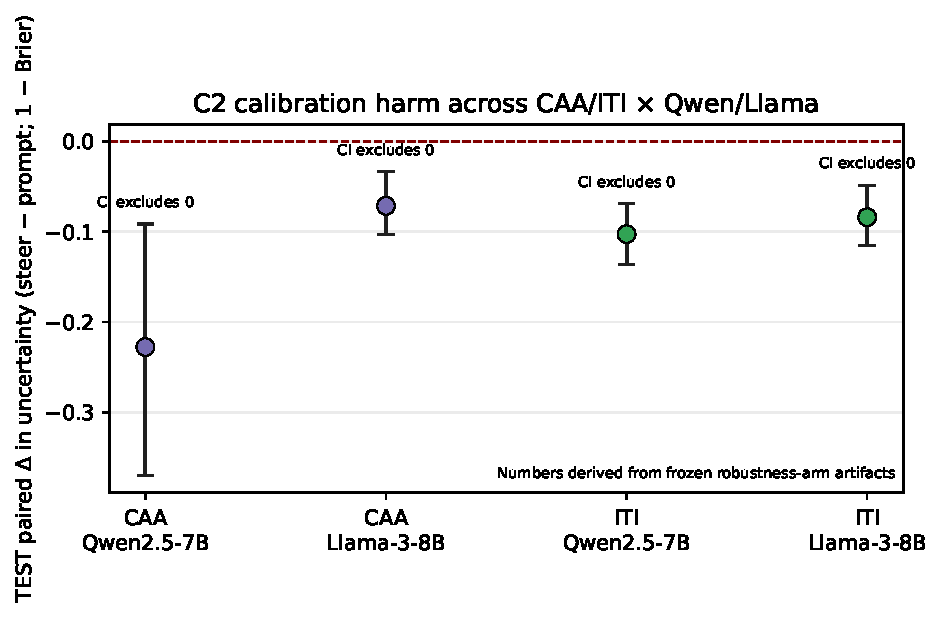
\includegraphics[width=\linewidth]{../figures/c2-calibration-harm.pdf}
\caption{Paired steer-minus-bounded-prompt uncertainty effects and Bonferroni-corrected intervals across the four tested model–method cells.}
\Description{All four uncertainty point estimates are negative relative to the selected prompt comparator, and their intervals exclude zero under the frozen scorer. The figure does not show direct steer-versus-unsteered-baseline harm or resolve missingness.}
\label{fig:c2-calibration-harm}
\end{figure}

In the Qwen--CAA format-and-missingness recheck, steering remained close to the unsteered baseline---about \(+0.011\) in parseable-confidence rate and \(+0.0008\) in \(1-\mathrm{Brier}\)---while the comparator scored higher under the reported outcome. {}% FL-044
{}% BD-009
The three-way comparison therefore supports a comparator-relative warning, not a claim that steering directly harmed baseline calibration.

The format-and-missingness recheck exposes a reporting confound: the parseable-confidence rate was 0.826 for steering and 0.445 for the prompt condition. {}% FL-045
Among complete pairs, steer minus prompt was \(-0.337\) with a 95\% confidence interval of \([-0.508,-0.165]\), but this analysis conditions on post-generation parseability, its adversarial all-generation bound widens to \([-0.478,+0.250]\) and crosses zero, and the other three uncertainty cells did not receive this recheck. {}% FL-046
{}% FL-047
{}% FL-048
{}% FL-049
The sign is therefore not identified under unrestricted missingness, and no grid-wide resolved uncertainty effect follows. {}% C-005

\begin{table*}[t]
\centering
\small
\caption{The calibration interpretation changes with comparator and missingness scope in the Qwen--CAA format-and-missingness recheck.}
\label{tab:calibration-scope}
\begin{tabular}{@{}p{0.27\textwidth}p{0.27\textwidth}p{0.36\textwidth}@{}}
\TopRule
Quantity & Reported value & Defensible interpretation \\
\midrule
Steer minus unsteered compliance & about $+0.011$ & Steering is near the unsteered baseline in this lineage. \\
Steer minus unsteered $1-\mathrm{Brier}$ & about $+0.0008$ & The steer-versus-prompt gap cannot be described as direct baseline harm. \\
Parseable-confidence rate & steer 0.826; prompt 0.445 & Conditions differ in confidence reporting. \\
Complete-case steer minus prompt & $-0.337\ [-0.508,-0.165]$ & Negative only among pairs where both outputs are complete. \\
All-generation adversarial bound & $[-0.478,+0.250]$ & Sign is not identified under unrestricted missingness. \\
Other uncertainty cells & not rechecked & No grid-wide format/missingness conclusion. \\
\bottomrule
\end{tabular}
% FL-044--FL-049
\end{table*}

\subsection{The Verdict Persists Across Five Split Seeds}\label{the-verdict-persists-across-five-split-seeds}

The reported no-pass verdict recurred over five split seeds. {}% FL-007
The original split had already been observed before four additional splits were prospectively frozen, and all splits reused the same item pool. {}% FL-035
The consistent outcome shows that the decision is not tied to one DEV/TEST partition.

% PENDING HUMAN RESULTS: populate H-F rows only from a frozen HUMAN_STUDY_PENDING.md packet.

% PENDING COMPOSITION RESULTS: populate P-F rows only from a frozen PROMPT_STEER_PENDING.md packet.

The procedure therefore returns more than pass or no-pass: it connects each evidence profile to a next diagnostic or design action. {}% OI-014

\section{Interface-Facing Qualification Record}\label{interface-facing-qualification-record}

\subsection{From Evaluation Output to Affordance State}\label{from-evaluation-output-to-affordance-state}

The record prevents three substitutions in interface reasoning: READ for TRANSFER, absolute output change for comparison against the declared alternative, and evidence from one tier for another. It binds those obligations to one proposed state: \emph{Diagnostic-only}, \emph{Unresolved}, \emph{Unstable}, or \emph{Eligible}. The mapping is applied here as a worked author synthesis; its validation boundary is consolidated in Limitations.

\subsection{Worked Record: Qwen--CAA Uncertainty}\label{worked-record-qwencaa-uncertainty}

\begin{table*}[t]
\centering
\footnotesize
\caption{Worked five-field record for Qwen--CAA uncertainty under the current evidence.}
\label{tab:worked-record}
\begin{tabular}{@{}p{0.19\textwidth}p{0.72\textwidth}@{}}
\TopRule
Field & Worked entry \\
\midrule
READ & Exploratory CAA-style READ satisfies the reported facade criterion for uncertainty on Qwen; one run, no ITI transfer. \\
TRANSFER & No-pass relative to the DEV-selected prompt comparator. \\
COMPARATOR & DEV-selected prompt from a preregistered bounded set of sixteen candidates; provenance limits follow the Method definition. \\
CALIBRATION WARNING & Steering is near the unsteered baseline in the one rechecked lineage; complete-case steer-minus-prompt remains negative, but adversarial all-generation missingness bounds cross zero and three cells are unrechecked. \\
EVIDENCE TIER & Qwen2.5-7B-Instruct, CAA single-layer additive intervention at hidden-state layer 20 (decoder-block-19 output hook at every token position), uncertainty task/outcome, seed 20260723, reported substitution protocol. \\
\bottomrule
\end{tabular}
% FL-003, FL-008, FL-009, FL-011, FL-024, FL-036, FL-038, FL-040, FL-042, FL-044, FL-047, FL-048, FL-080, FL-081
\end{table*}

Under the proposed mapping, this record is \emph{Unresolved}: the TRANSFER test is no-pass relative to the comparator and the all-generation contrast remains partially identified. {}% C-005
{}% C-007
Local READ evidence still supports inspection.

\subsection{Illustrative Design Scenario}\label{illustrative-design-scenario}

Return to Alex's policy-writing assistant. The prototype uncertainty slider has local Qwen--CAA READ support, but its TRANSFER record is no-pass relative to the comparator. The targeted recheck shows steering near the unsteered baseline, a negative complete-case steer-minus-prompt estimate, and missingness bounds that cross zero. {}% FL-044
{}% FL-047

For this record, the team withholds the active slider and keeps a read-only inspection trace. The comparator view explains what the prompt channel achieved; the warning distinguishes steer-versus-prompt from steer-versus-baseline; and the evidence tier keeps the Qwen--CAA result from migrating to ITI or Llama.

\begin{figure*}[t]
\centering
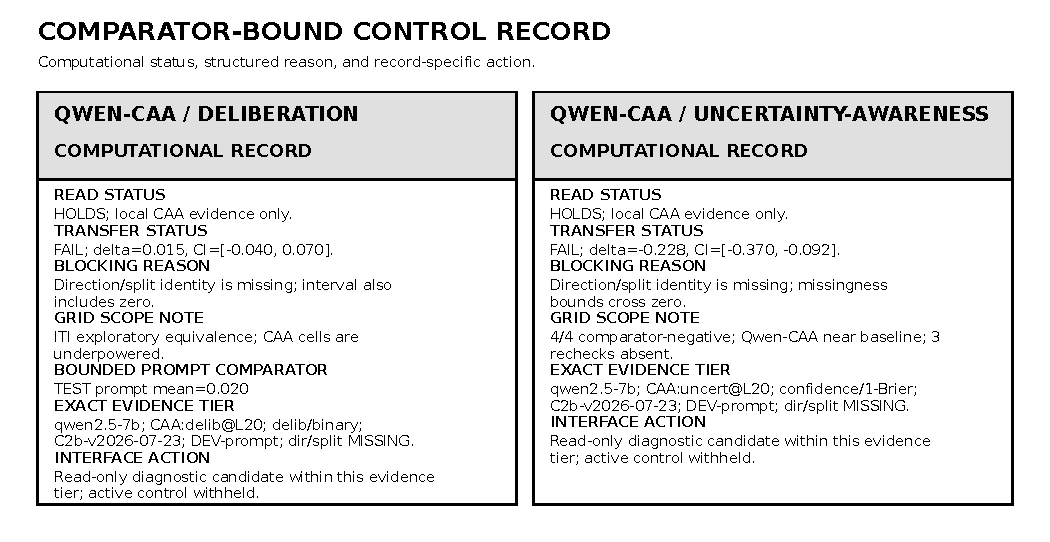
\includegraphics[width=\textwidth]{../figures/console-ui-contract.pdf}
\caption{Artifact-derived cards make the comparator, evidence profile, tier, and next design action visible.}
\Description{Two console cards summarize deliberation and uncertainty. Deliberation is unresolved because evidence is mixed; uncertainty is unresolved because the comparator-relative result is limited by missingness. The uncertainty design action withholds one active slider while retaining diagnostic and comparator information.}
\label{fig:console}
\end{figure*}

\subsection{Display Requirements Implied by the Record}\label{display-requirements-implied-by-the-record}

An interface that exposes this record would need to keep the relative comparison visible. Showing only the negative steer-minus-prompt estimate could imply that steering harmed baseline calibration; the Qwen--CAA format-and-missingness recheck instead places steering near baseline and the comparator above it. {}% FL-044
The record must also expose missingness rather than letting a complete-case interval stand in for all generations. {}% FL-046
{}% FL-049
Finally, the evidence tier must prevent Qwen--CAA READ from appearing as evidence for Llama, ITI, another layer, or another task.

Human-AI guidelines support communicating capabilities and limitations, while interpretability-tool studies show the value of making the basis of a judgment inspectable. \cite{amershi2019guidelines,kaur2020interpreting} The record therefore exposes the reason for a state rather than presenting a green or red badge.

% PENDING HUMAN INTERFACE RESULT: replace from HUMAN_STUDY_PENDING.md only.

\section{Discussion}\label{discussion}

\subsection{READ Supports Inspection Without Presuming Actionability}\label{read-supports-inspection-without-presuming-actionability}

A readable direction can still support inspection, debugging, hypothesis formation, or a read-only trace. The worked READ results make that value concrete: deliberation and skepticism satisfy the facade criterion in both model families, while uncertainty and focus differ by model. {}% FL-039
{}% FL-040
The alternative is not ``ship a slider'' or ``hide the representation.'' It is to preserve local evidence without turning visibility into a behavioral promise.

The three evidence profiles point to different actions. Skepticism requests more resolution; deliberation calls for a better-targeted test; uncertainty calls for measurement repair and a comparator-specific warning. {}% FL-041
{}% FL-043
{}% FL-047
This translation from evidence profile to interface action is the record's practical contribution.

\subsection{Why the Comparator Changes the Interface Claim}\label{why-the-comparator-changes-the-interface-claim}

An active latent control makes a claim about consequences, not merely movement. In the Qwen--CAA format-and-missingness recheck, the comparator field identifies prompt improvement over a steer-near-baseline condition rather than direct steering harm. {}% FL-044
{}% FL-045
The comparator changes what the same observed gap means for the interface.

The procedure asks designers to disclose the comparator rather than canonize it. In this application, the comparator is the DEV-selected prompt defined in Method. {}% FL-008
{}% FL-009
{}% BD-009
The procedure also distinguishes substitution from deployment: the present experiment replaces that prompt with steering, whereas a user-facing slider normally acts on top of an instruction. {}% FL-015

% PENDING PROMPT-PLUS-STEER DISCUSSION: choose P-A through P-E and revise construct scope.

\subsection{Qualification Is a Versioned Lifecycle}\label{qualification-is-a-versioned-lifecycle}

A new model, method, direction, comparator, item pool, or interface version creates a new evidence tier rather than inheriting the current result. This lifecycle keeps the artifact useful without treating a local classification as permanent or universal.

% PENDING HUMAN DISCUSSION: choose H-A through H-E; preserve null/adverse/incomplete evidence.

\section{Limitations, Ethics, and Future Work}\label{limitations-ethics-and-future-work}

\subsection{Evidence Provenance and Reproducibility}\label{evidence-provenance-and-reproducibility}

The repository contains the core result directories, frozen preregistrations, executable adjudicator, evidence ledger, paper manifests, generated tables and figures, and independent audit summaries. {}% OI-001
The committed JSON artifacts can regenerate the claim-bearing paper tables and figures without GPU access. The author-proposed affordance-state assignments remain non-generated judgments and have not been independently reproduced.

The available lineage records exact layers, hook convention, contrast splits, prompt wrappers, generation defaults, TEST denominators, split seeds, and degradation scorer. {}% FL-075
{}% FL-080
Remaining reproducibility limits include immutable upstream model revision hashes and incomplete environment/data hashes in the older E-0006 registry entries; reproducing raw generations therefore requires reconstructing those model snapshots and software environments, whereas regenerating the paper artifacts uses the committed result JSON and manifests.

\subsection{Assay Validity and Statistical Resolution}\label{assay-validity-and-statistical-resolution}

Because no latent behavioral positive control passes, the no-pass grid cannot distinguish a true absence of actionability from limitations in direction construction, scale, hook/layer selection, normalization, generation, outcome, or scoring. {}% FL-057
Prompt endpoint liveness and random-direction sensitivity show that parts of the pipeline respond; they do not validate the target intervention. The raw-magnitude follow-up narrows simple under-scaling only for Qwen single-layer CAA, and CAA/ITI coefficients do not imply a common injected norm. {}% FL-026
{}% FL-054
{}% FL-078

The diagnostic studies provide supporting context: a direct refusal prompt reaches 95.5\%, a random uncertainty direction shifts the measured outcome by \(-0.24\) with 95\% CI \([-0.36,-0.12]\), bounded CAA produces 0\% refusal, and the raw-magnitude Qwen--CAA sweep produces no qualifying nondegenerate pass. {}% FL-051
{}% FL-052
{}% FL-055
The preregistered whitened-Mahalanobis analysis also returns no support for the tested off-manifold mechanism. {}% FL-050
The first-token logit analysis remains non-claim-bearing appendix context.

Resolution also differs by claim. READ is exploratory, single-run, and CAA-specific. {}% FL-036
{}% FL-038
Skepticism is underpowered relative to the point-estimate floor, deliberation's equivalence descriptions are post hoc, and uncertainty remains format- and missingness-sensitive. {}% FL-041
{}% FL-043
{}% FL-047
{}% FL-048
Five split seeds over one item pool address partition sensitivity rather than replication, and within-cell correction does not establish a familywise global null across the grid. {}% FL-034
{}% FL-035

\subsection{Comparator, Substitution, and Interface Construct}\label{comparator-substitution-and-interface-construct}

The prompt comparator is selected on DEV from a preregistered bounded candidate set. Its authorship independence, TEST blindness, and resource parity are not established; a different candidate set or search budget could change the contrast. {}% BD-009
{}% OI-012
Conclusions therefore remain relative to this declared alternative.

The application substitutes steering for the selected prompt, whereas a product control would ordinarily act in the presence of a user's instruction. {}% FL-015
Prompt-plus-steer evidence is pending, so the paper makes no composition claim. {}% OI-004
{}% OI-017
The four-state mapping was synthesized from the observed evidence profiles rather than frozen in advance, and no independent analyst reproduced its assignments. {}% FL-076
{}% FL-077

\subsection{Human Evidence, Ethics, and Future Validation}\label{human-evidence-ethics-and-future-validation}

The current study contains no human result, so the paper does not claim that people understand the record, calibrate reliance, or make better control-granting decisions. {}% OI-003
{}% OI-016
Any future human evaluation requires the applicable ethics determination, consent and recruitment records, compensation, exclusion flow, and privacy handling.

The state mapping is an author-proposed post hoc synthesis rather than an independently reproduced rubric. A structured record can create false assurance when its comparator, measurement, or assignment is treated as universal; the record therefore displays its evidence tier and warning. Human evaluation should separately measure comprehension, decision calibration, behavior, and perceived helpfulness. \cite{karny2026neural,bucinca2021trust}

\section{Conclusion}\label{conclusion}

A latent control should not be licensed by readability or output movement alone. The comparator-bound contract asks whether the intervention improves the named behavior over a declared alternative, then preserves READ, TRANSFER, comparator, calibration warning, and evidence tier in the interface decision.

In the tested Qwen/Llama and CAA/ITI setting, the contract separates one aggregate no-pass result into three useful decisions: increase resolution for skepticism, preserve mixed deliberation evidence, and attach a comparator-specific calibration warning to uncertainty. In the worked uncertainty scenario, that distinction supports a concrete action---retain diagnostic evidence, expose the comparator and warning, and withhold one unsupported slider. The contribution is a practical interface rule: evidence determines the affordance, and each new evidence tier earns its own decision.

\appendix

\section{Author-Proposed Assignment Checklist}\label{author-proposed-assignment-checklist}

The checklist makes the proposed procedure inspectable; it does not supply independent or inter-rater validation.

\begin{enumerate}
\def\labelenumi{\arabic{enumi}.}
\tightlist
\item
  \textbf{Specify candidate and tier.} Record model, method, direction construction, layer, task, version, and protocol.
\item
  \textbf{Define outcome and READ evidence.} State what behavior the proposed control names and whether local representational evidence supports the label.
\item
  \textbf{Declare the behavioral alternative.} Record comparator set, selection procedure, budget, and known provenance limits without calling it fair or optimal.
\item
  \textbf{Run TRANSFER and coherence.} Report paired estimand, uncertainty rule, point-estimate floor, missingness, exclusions, and coherence result.
\item
  \textbf{Issue a provisional state.} Assign exactly one formal state---\emph{Diagnostic-only}, \emph{Unresolved}, \emph{Unstable}, or \emph{Eligible}---and attach its reason, comparator, warning, and evidence tier.
\end{enumerate}

Any model, method, axis, layer, task, comparator, outcome, or protocol change creates a new record. {}% FL-077

\section{Non-Claim-Bearing Logit Diagnostic}\label{non-claim-bearing-logit-diagnostic}

This diagnostic is qualitative context and is excluded from claim support. It uses five probes per axis and measures first-position log-sum-exp changes for refusal-leading tokens, including tokens such as ``I'' that may begin ordinary or hedged answers. {}% FL-058
At coherent \(\beta=1\), the refusal direction raises this token mass by about 13.9 nats on average while 0 of 5 probes match the refusal markers. One probe rises by about 16.9 nats with a byte-identical greedy completion; at \(\beta=2\), generation becomes repetitive. {}% FL-059
{}% FL-060
Token-proxy movement is not scored refusal and does not establish a working latent handle.

\begin{acks}
Acknowledgements omitted for anonymous review.
\end{acks}

\bibliographystyle{ACM-Reference-Format}
\bibliography{reframed-references}

\end{document}